%
\documentclass[12pt]{article}%
\usepackage[utf8]{inputenc}
\usepackage[T1]{fontenc}

%%%Margins and Indent 
\setlength{\parindent}{-1pt}
\usepackage{geometry}
\geometry{
 a4paper,
 total={170mm,257mm},
 left=15mm,
 right = 15mm,
 bottom=15mm ,
 top=15mm,}
 
\usepackage{hyperref}

 %%% Font
\usepackage{amsmath,accents}


%%% images
\usepackage{graphicx}
\usepackage{caption,subcaption}

%%Algorithm
\usepackage[commentsnumbered]{algorithm2e}
%\usepackage{algpseudocode}

\numberwithin{equation}{section}
\usepackage{tabularx,multirow}

%%Tikz 
\usepackage{tikz}
\usetikzlibrary{angles, quotes, calc, decorations.markings, intersections}
\newcommand{\midlabelline}[3]{
   \node (midlabel) at ($ (#1)!.5!(#2) $) {#3};
   \draw[<-] (#1) --  (midlabel);
   \draw[->] (midlabel) -- (#2);
}

%%import
\usepackage{import}
\usepackage{xifthen}
\usepackage{pdfpages}
\usepackage{transparent}

%%%%defined commands
\newcommand{\pa}{\partial}
\newcommand{\mcm}[1]{\mathcal{#1}}
\newcommand{\bo}{\mcm{O}}
\newcommand{\sDelta}{{\scriptstyle \Delta}}
\newcommand{\gs}{\hspace{0.35cm}}
\newcommand{\mvec}[1]{\accentset{\rightharpoonup}{#1}}
 
%%%%%%%%%%%
\begin{document}

\abstract{}
%\centering{\Large{Abstract}}}

In this project will try to solve poisson equation for interleaved capacitor computationally using the method of finite differences to convert them into a system of linear equation and then using iterative schemes like SOR, Gauss Seidel Method , Jacobi Method , SOR (Successive Over Relaxation ) Method. We would also like to develop intuiton for poisson equation related problems related to electrostatic potential and compare the different iterative schemes named above on the basis of number of iterations to find the most compuationally viable method.We would also like to discuss the topics such as truncation error and non dimensionalisation which are involved in coverting the physical poisson  problem into computational problem.
\newpage
\tableofcontents
\newpage
	\section {Introduction}
    \subsection{Motvation}
    \noindent 
    We first encountered Laplace Equation during our course in electricity and magnetism in second semester and we were fascinated with how one can calculatge the potential in a region just by knowing the boundary condition, ofcourse the region has to be charge free for applying Laplace Equation. After Laplace Equation , we were introduced to Poisson Equation which we were able to solve for region having charges( or sources ). When we were given the oppurtunity to choose a project in our computational physics this semester, it did not take us long to decide the topic for project.
    \subsection{General Idea}
    In our project we will try to tackle the Laplace and Poisson equaton which is an ellipitic linear partial differential equation having application in various fields of physics ranging from thermodynamics, electrostatics etc. We will solve the equation computationally using the method of finite differences in one and two dimensions for rectangular membrane. We will first convert the partial differential equation into system of linear differential equation and then use three different iteration schemes for solving those system of linear equation.\\ 
    \subsection{Poisson and Laplace Equation}
    	The general form of Poisson's equation in Euclidean space is given here,
    \[
    \scalebox{1.3}{$\vec{\nabla}^2 \varphi(\vec{r}) = f(\vec{r})$}
    \]
    where, $f(\vec{r})$, $\varphi(\vec{r})$ are the functions of position vector $\vec{r}$. $f(\vec{r})$ is given and $\varphi(\vec{r})$ is sought. \\
    In our case  $\varphi(\vec{r})$ is electrostatic potential, $ f(\vec{r})$ is the charge density of region in which solution is required. In a special case in which  $f(\vec{r}) = 0 $ we can apply same process for solving laplace equation for a region free of charge.
    \subsection{Plan of Report}
    In theory section we will formulate and explain the physical problem we chosen to solve using finite difference method. In methodology we will explain our methods and explain the algorithm followed for programming. In the Result and anlaysis section we analyse our results compared to what we expect to obtain and also compare different iterative methods based on our computation relating problem.And in computation we would like to discuss our experiences and results in brief.
\newpage
\section{Theory}
Identical infinitely-long thin metal plates $A_1,A_2,A_3,A_4,A_5,B_1,B_2,B_3 $ and $B_4$ are placed in an \textit{interleaved} arrangement as dipicted in fig1.(a) Group of plates $A_i$ and $B_i$ are connected to the terminal $A$ and $B$ , respectively, by means of gold wires. The terminals are connected to different potential sources $U_A$ and $U_B$ respectively. \\
This is called an interleaved capacitor, Our goal will be to approximate the potential distribution (in two dimensions considering symmetry along the the third axis which will be dropped) inside the capacitor after we disconnect the capacitor from sources, treating the interior plates as line charge distributions.
\begin{align*}
    &U_A = 5V \\
    &U_B = -5V \\
    &\text{Capacitance } = 0.1\mu F\\
    &\text{Distance between plates ($d$)} = 0.5\mu m \\
    &\textit{Dimensions: } 4 \times 4.4 \mu m  
\end{align*}
This arrangement can be seen as a number of parallel plate capacitors connected in parallel to each other as seen in fig1(b),
if $C_0$ is the capacitance of each capacitor in parallel and $C$ is the capacitance of the entire arrangement then,
\begin{align*}
    C_0 = C/8
\end{align*}
Also we know that for parallel plate capacitors with cross-section area $A$ and distance $d$ between the plates,
\begin{align}
    C_0 = \epsilon_0 \frac{A}{d} \implies A = \frac{C_0d}{\epsilon_0}
\end{align}
Therefore the charge distribution on any plate $A_i$ is given by,
\begin{align}
    \rho_A = \frac{(C \times V )}{5A} \implies \rho_A = 2\epsilon_0 \times 10^5C m^{-2} 
\end{align}
Similarly on $B_i$,
\begin{align}
    \rho_B = -2\epsilon_0 \times 10^5C m^{-2} 
\end{align}

\begin{figure}[h]
    \centering
    \begin{subfigure}[b]{\linewidth}
    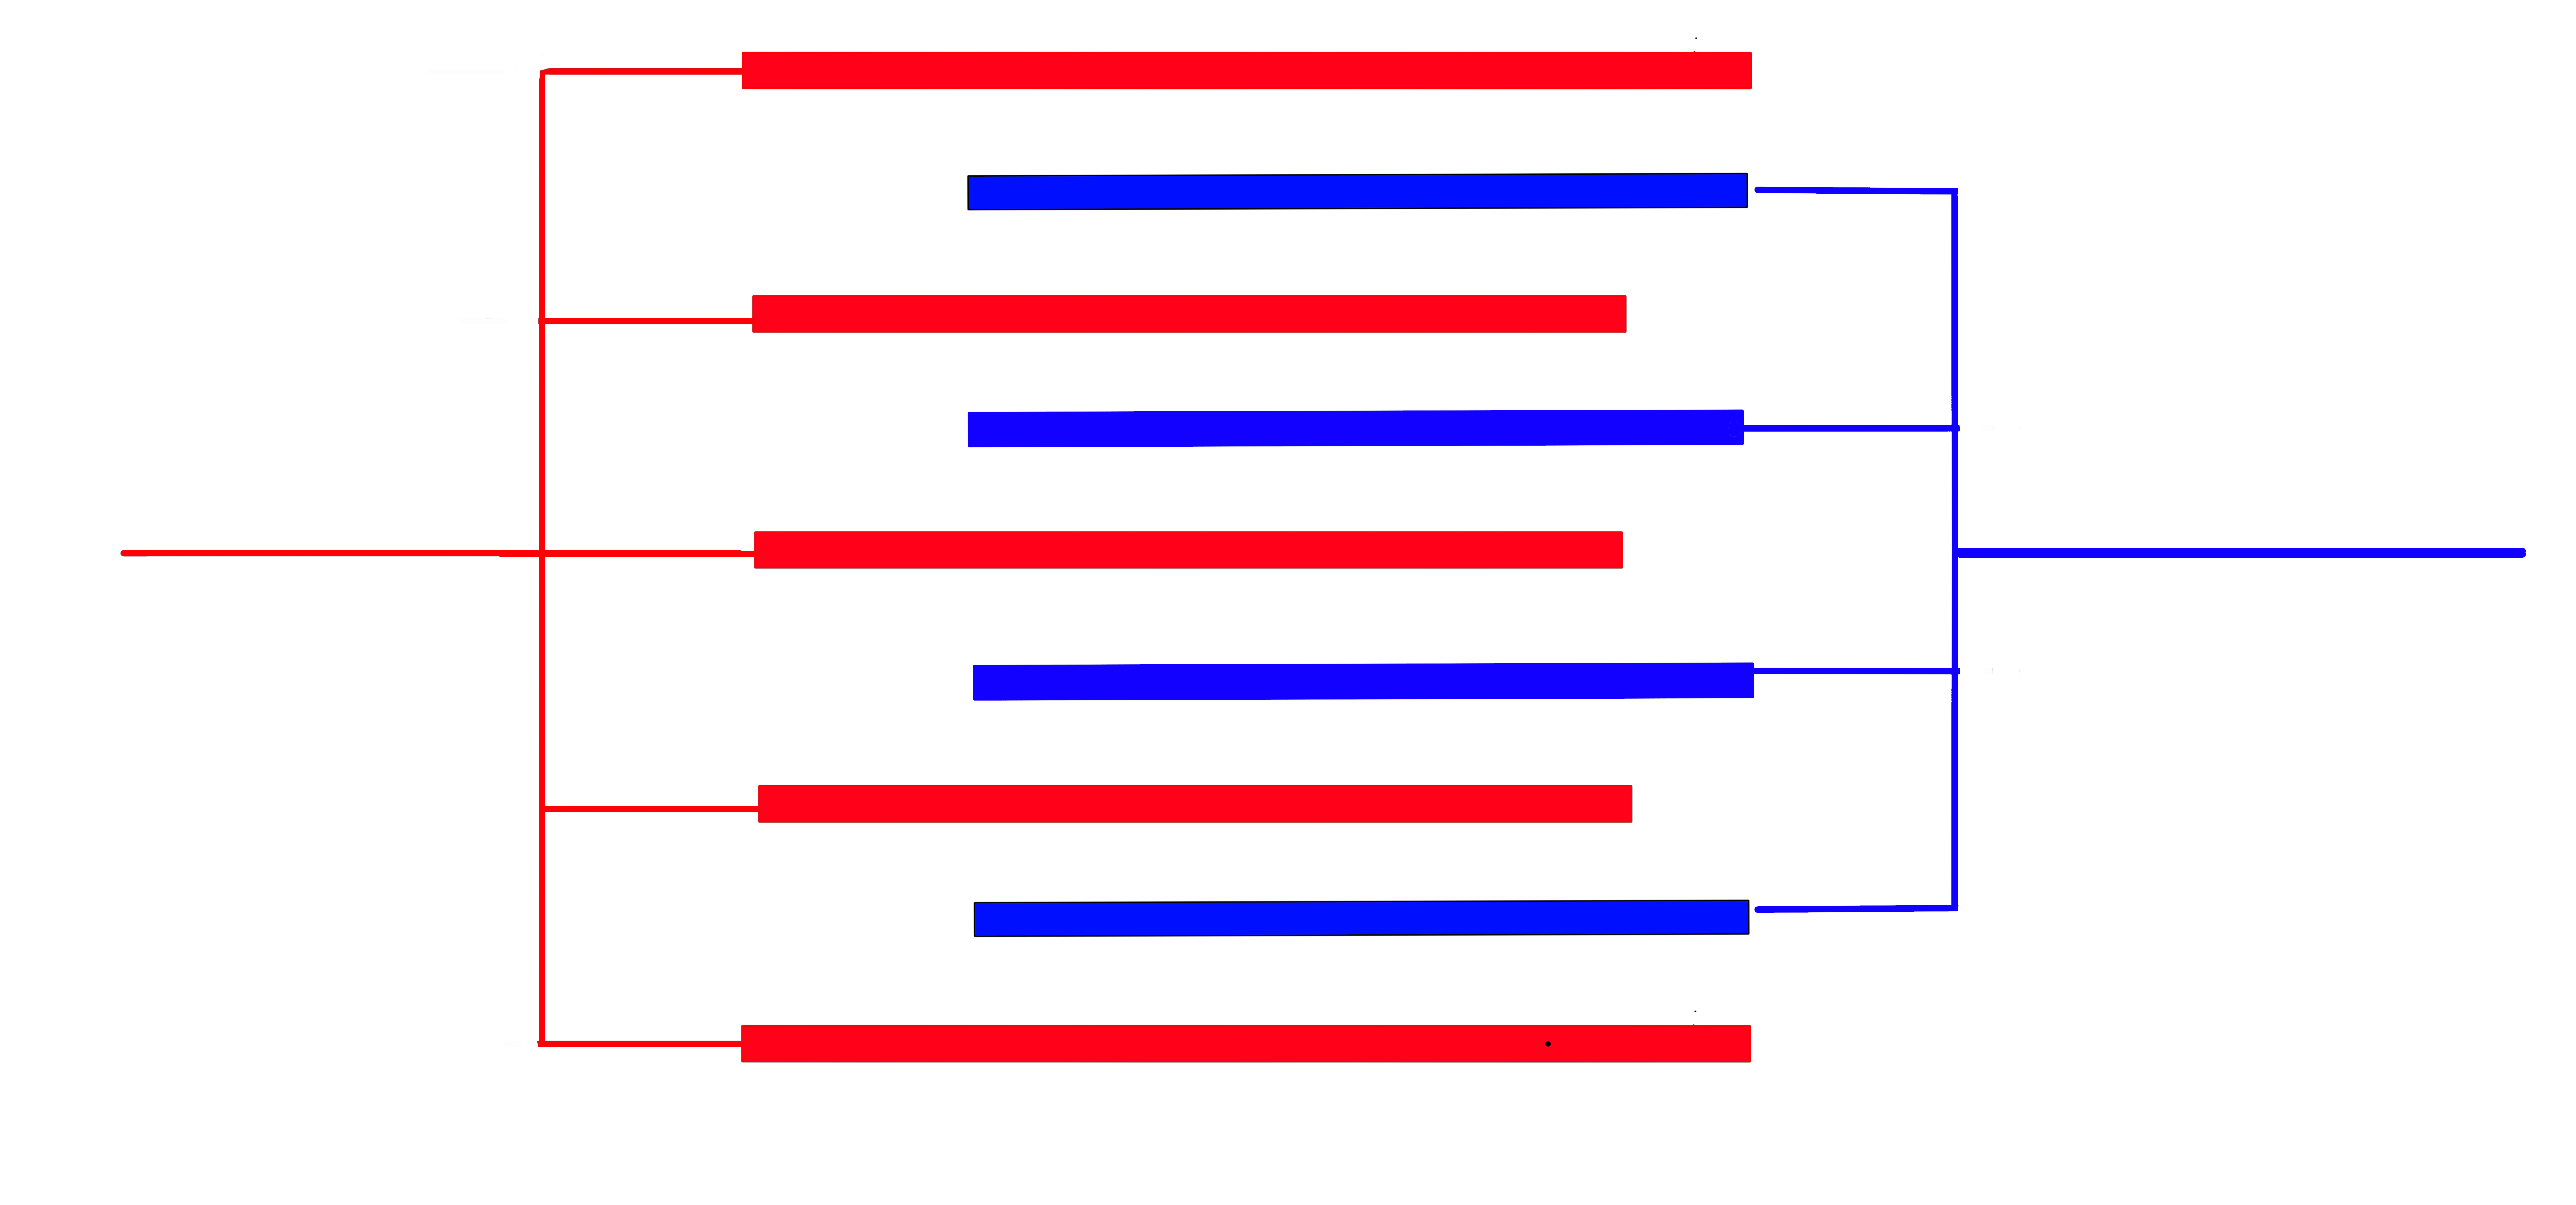
\includegraphics[width=0.5\textwidth, height=4cm]{content/capacitor.png}
    \caption{\small Diagram dipciting the arrangement of plates in a interleaved fashion.}
    \label{fig 1: the capacitor}
    \end{subfigure}
\end{figure}

\begin{figure}[h]
    \centering
    \def\svgwidth{0.6\textwidth}
    \import{./diagrams}{daigram.pdf_tex}
    \caption{Riemmans theorem}
    \label{fig:riemmans-theorem}
\end{figure}

Mathematical Formulation:\\
Let $U(x,y)$ and $\vec{E}(x,y)$ be the potential and Electric field distribution defined in the region of our arrangement $(x,y) \in \Omega := [0,4\mu m]\times[0,4.4\mu m]$ .\\
We know from maxwell's laws that for static electric fields $\vec{\nabla} \cdot \vec{E} = \rho / \epsilon_0 $, $\vec{\nabla} \times \vec{E} = 0$
\\
From the later we get $E=-\vec{\nabla}U$, substituting this back into the former we get,
\begin{equation*}
    \vec{\nabla}^2 U = \frac{-\rho}{\epsilon_0}  
\end{equation*}
In two dimensions with euclidean coordinate system the equation reduces to, 
\begin{equation}
    \frac{\pa^2U(x,y) }{\pa x^{2}} + \frac{\pa^2U(x,y) }{\pa y^{2}}= -\frac{\rho(x,y)}{\epsilon_0} \\
\end{equation}
where,
\begin{equation}
\rho(x,y) =  \begin{cases}
    -2\epsilon_0 \times 10^5 C m^{-2} & :\text{if} \gs (x,y) \in B_i \gs \text{where} \gs i = 1,2,3,4 \\
    2\epsilon_0 \times 10^5 C m^{-2} & :\text{if} \gs (x,y) \in A_i \gs \text{where} \gs i = 2,3,4  \\
    0 C m^{-2} & : \gs \text{elsewhere}
\end{cases}  
\end{equation}
Now according to our given arrangement,
\begin{align}
    B_1 &= \{ (x^*,y^*) \gs : \gs x^*= 0.5\mu m \gs;\gs 0.4\mu m \leq y^* \leq 4.4\mu m \} \\
    B_2 &= \{ (x^*,y^*) \gs : \gs x^*= 1.5\mu m \gs;\gs 0.4\mu m \leq y^* \leq 4.4\mu m \} \\
    B_3 &= \{ (x^*,y^*) \gs : \gs x^*= 2.5\mu m \gs;\gs 0.4\mu m \leq y^* \leq 4.4\mu m \} \\
    B_4 &= \{ (x^*,y^*) \gs : \gs x^*= 3.5\mu m \gs;\gs 0.4\mu m \leq y^* \leq 4.4\mu m \} \\
    A_2 &= \{ (x^*,y^*) \gs : \gs x^*= 1\mu m \gs;\gs 0\mu m \leq y^* \leq 4\mu m \} \\
    A_3 &= \{ (x^*,y^*) \gs : \gs x^*= 2\mu m \gs;\gs 0\mu m \leq y^* \leq 4\mu m \} \\
    A_4 &= \{ (x^*,y^*) \gs : \gs x^*= 3\mu m \gs;\gs 0\mu m \leq y^* \leq 4\mu m \} 
\end{align}
We get the following boundary conditions for the above boundary value problem,
\begin{align}
    & U(0,y) = +5 V \gs; \gs U(4,y) = +5 V \\ 
    & U_y(x,0) = 0V/m \gs; \gs U_y(x,4.4) = 0V/m 
\end{align}

Non-Dimensionalizing the variables,

Let new dimensionless variables,
\begin{align}
    x' = \frac{x}{s} \gs \gs y' = \frac{y}{s} \gs \gs U' = \frac{U}{\nu}
\end{align}
where $s$ and $\nu$ are known constant scaling factors having dimensions of length and electric potential respectively.

The B.V.P reduces to,
\begin{equation}
    \frac{\pa^2U'(x',y') }{\pa x^{'2}} + \frac{\pa^2U'(x',y') }{\pa y^{'2}}= -\frac{\rho'(x',y') s^2}{\epsilon_0 \nu} \\
\end{equation}
where,
\begin{equation}
\rho'(x',y') =  \begin{cases}
    -2\epsilon_0 \times 10^5  & :\text{if} \gs (x',y') \in B_i \gs \text{where} \gs i = 1,2,3,4 \\
    2\epsilon_0 \times 10^5 & :\text{if} \gs (x',y') \in A_i \gs \text{where} \gs i = 2,3,4 \\
    0  & : \gs \text{elsewhere}
\end{cases}
\end{equation}
Now according to our given arrangement,
\begin{align}
    B_1 &= \{ (x^*,y^*) \gs : \gs x^*= 0.5/s \gs;\gs 0.4/s \leq y^* \leq 4.4/s \} \\
    B_2 &= \{ (x^*,y^*) \gs : \gs x^*= 1.5/s \gs;\gs 0.4/s \leq y^* \leq 4.4/s \} \\
    B_3 &= \{ (x^*,y^*) \gs : \gs x^*= 2.5/s \gs;\gs 0.4/s \leq y^* \leq 4.4/s \} \\
    B_4 &= \{ (x^*,y^*) \gs : \gs x^*= 3.5/s \gs;\gs 0.4/s \leq y^* \leq 4.4/s \} \\
    A_2 &= \{ (x^*,y^*) \gs : \gs x^*= 1/s \gs;\gs 0/s \leq y^* \leq 4/s \} \\
    A_3 &= \{ (x^*,y^*) \gs : \gs x^*= 2/s \gs;\gs 0/s \leq y^* \leq 4/s \} \\
    A_4 &= \{ (x^*,y^*) \gs : \gs x^*= 3/s \gs;\gs 0/s \leq y^* \leq 4/s \} 
\end{align}
We get the following boundary conditions for the above boundary value problem,
\begin{align}
    & U(0,y) = +5/\nu \gs; \gs U(4,y) = +5/\nu \\ 
    & U_y(x,0) = 0 \gs; \gs U_y(x,4.4) = 0 
\end{align}

%%%%%%%%%%%%%%%END%%%%%%%%%%%%%%%%%%%%%%
\newpage
\section{Methodology}
\subsection{Finite Difference Method}
Finite Difference Methods(FDM) are used for approximating the solution of partial differential equations over a set of finite points, arranged in a geometrical structure called a \textbf{mesh}%
\footnote[1]{An object which consists of points which are spaced in a specific geometrical pattern is referred to as a \textbf{mesh} and each point in this mesh is called a \textbf{node}. The distance between any two adjacent nodes in a mesh with uniform spacing is called its \textbf{meshsize}}%
, in the continous domain of solution. The methods involve the idea of reducing the given PDE, by means of truncated taylor series approximation of the derivatives, to a difference equation which is much easier to digest numerically. 
\subsubsection{Finite Difference Approximations}
The quality of the solution depends on the quality of approximations made to the derivatives.
%%%
Consider this one-dimensional structured mesh of nodes $(x_0,x_1,x_2,..,x_i,..,x_n)$ at which the solution $U(x_i)$  is to be found, such that the difference $h = x_{i+1} - x_i $ is constant throughout the mesh and $x_i \equiv x_0 + ih$.\\
\begin{figure}[h]
\centering

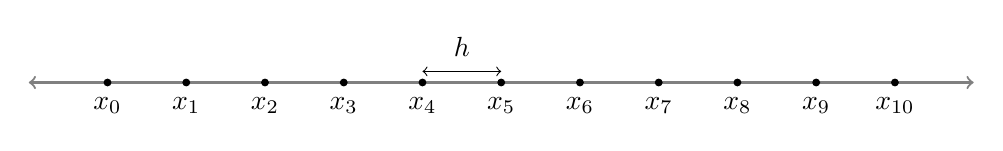
\begin{tikzpicture}
    \coordinate (H) at (4.5,6pt);
    \draw[thick,color=gray,<->] (-1,0) -- (11,0);
    \foreach \x  in {0,1,2,3,4,5,6,7,8,9,10}
        \draw[fill=black] (\x cm,0) circle (1.2pt) (\x cm,-2pt) node[anchor=north] {$x_{\x}$};
    \draw[thin,<->] (4,4pt) -- (5,4pt);%
    \node[anchor=south] at (H) {$h$};
\end{tikzpicture}

\caption{\small 1D mesh with 11 nodes and a meshsize h}
\end{figure}
\\
Let $U'_i$ represent the solution at the $i$-th node and \hfill
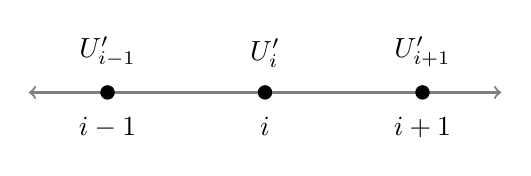
\begin{tikzpicture}[scale =2]
    \draw[thick,color=gray,<->] (3,-2cm) -- (6,-2cm);
    \foreach \x  in {3.5,4.5,5.5}
        \draw[fill=black] (\x cm,-2cm) circle (1.2pt) ;
    \draw (3.5 cm,-2.01cm) node[anchor=north,shift={(0,-5pt)}] {$i-1$};
    \draw (4.5 cm,-2.01cm) node[anchor=north,shift={(0,-5pt)}] {$i$};
    \draw (5.5 cm,-2.01cm) node[anchor=north,shift={(0,-5pt)}] {$i+1$};
    \draw (3.5 cm,-1.99cm) node[anchor=south,shift={(0,5pt)}] {$U'_{i-1}$};
    \draw (4.5 cm,-1.99cm) node[anchor=south,shift={(0,5pt)}] {$U'_{i}$};
    \draw (5.5 cm,-1.99cm) node[anchor=south,shift={(0,5pt)}] {$U'_{i+1}$};
\end{tikzpicture}
\begin{equation*}
    \left. \frac{\partial U}{\partial x} \right|_{x_ i} = U'_{x}(x_0 + ih) \equiv U'_{x}|_i
\end{equation*} 
\begin{equation*}
    \left. \frac{\partial^2 U}{\partial x^2} \right|_{x_ i} = U'_{xx}(x_0 + ih) \equiv U'_{xx}|_i
\end{equation*}

The first order derivative can be defined as,
{\raggedright 
\begin{align*}
    &\text{} \hspace{1cm} U'_x|_i = \lim_{h \to 0} \frac{U'_{i+1} - U'_i}{h}  \\
    &\text{or,} \hspace{1cm} U'_x|_i = \lim_{h \to 0} \frac{U'_{i} - U'_{i-1}}{h}  \\
    &\text{or,} \hspace{1cm} U'_x|_i = \lim_{h \to 0} \frac{U'_{i+1} - U'_{i-1}}{2h}  
\end{align*}
}

Finite difference approximations are obtained by dropping the limit and can be written as, 
 
\begin{flalign*}
    &\text{Forward Difference} \hspace{1cm} U'_x|_i \approx \frac{U'_{i+1} - U'_i}{h} \equiv \delta^+_{x} U'_i  \\
    &\text{Backward Difference} \hspace{1cm} U'_x|_i \approx \frac{U'_{i} - U'_{i-1}}{h} \equiv \delta^-_{x} U'_i \\
    &\text{Central Difference} \hspace{1cm} U'_x|_i \approx \frac{U'_{i+1} - U'_{i-1}}{2h} \equiv \delta_{2x} U'_i 
\end{flalign*}

Where $\delta^+_{x} , \delta^-_{x} , \delta_{2x}$ are called the \textbf{finite diference operators} for approximating \textbf{first-order derivatives} and their expansion is called the \textbf{finite difference quotient}, each representing forward,backward and centered respectively.
Second and Higher order finite difference Quotients can also be obtained,
\begin{align*}
    U'_{xx}|_i &= \lim_{h \to 0} \frac{U'_x(x_i+\frac{h}{2}) - U'_x(x_i-\frac{h}{2})}{h} \\
    &= \lim_{h \to 0} \frac{1}{h} \left[{\frac{U(x+h) - U(x)}{h} - \frac{(U(x)- U(x-h))}{h}}\right]\\
    &= \lim_{h \to 0}\frac{U'_{i+1}-2 U'_i + U'_{i-1}}{h^2} \\
    &\approx \boxed{\delta^2_x U'_i \equiv \frac{1}{h^2}(U'_{i+1}-2 U'_i + U'_{i-1})} \hspace{1cm} \text{[Central second-order Difference]}
\end{align*}

\begin{figure}[h]
    \centering
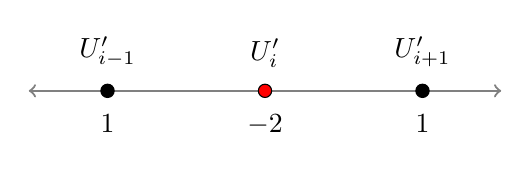
\begin{tikzpicture}[scale=2]
    \coordinate (A) at (3.5 cm,0cm);
    \coordinate (B) at (4.5 cm,0cm);
    \coordinate (C) at (5.5 cm,0cm);
    \draw[thick,color=gray,<->] (3cm,0) -- (6cm,0);
    \draw[fill=black] (A) circle (1.2pt) (A) node[anchor=north,shift={(0,-5pt)}] {$1$};
    \draw[fill=red] (B) circle (1.2pt) (B) node[anchor=north,shift={(0,-5pt)}] {$-2$};
    \draw[fill=black] (C) circle (1.2pt) (C) node[anchor=north,shift={(0,-5pt)}] {$1$};
    \draw (A) node[color=black,anchor=south,shift={(0,5pt)}] {$U'_{i-1}$};
    \draw (B) node[color=black,anchor=south,shift={(0,5pt)}] {$U'_{i}$};
    \draw (C) node[color=black,anchor=south,shift={(0,5pt)}] {$U'_{i+1}$};
\end{tikzpicture}
\end{figure}

The vector of coefficients of the function values at various nodes forms what is called the \textbf{stencil} of the finite difference operator and it uniquely idetifies the operator. The combination $(1,-2,1)$ is called a \textbf{three point stencil} as it combines function values from three different points on the mesh.
It is fairly obvious to notice that any finite difference operator for any derivative at any node is just a linear combination of the function values at various neighbourhood nodes.   

\subsubsection{Local Truncation Error of Finite Difference Approximations}
The \textit{'error'} that accompanies \textit{'approximations'} in the method must be acccounted for. In this section, the truncation error in the derivative approximations is ascertained which will later help us deduce the error in PDE's solved using these approximations.
\\[2mm]
\textbf{The local truncation error for derivative approximations} is defined here as the difference between the exact value of the derivate and the approximated value at node $i$, it can be calculated using Taylor series expansions about $i$,\\[2mm]
For Forward difference operator, 
\begin{align*}
    \tau &\equiv \delta _ x^{+} U'_ i - {U'_ x}|_ i \\
    &= \frac{1}{\sDelta x}\left( U'_ {i+1} - U'_{i}\right) - {U'_ x}|_i \\
    &= \frac{1}{\sDelta x}\left[ \left( U'_ i + \sDelta x{U'_ x}|_ i + \frac{1}{2}\sDelta x^2{U'_{xx}}|_ i + \mcm{O}(\sDelta x^3)\right) - U'_i \right] - {U'_ x}|_ i \\
    &= \frac{1}{2}\sDelta x{U'_{xx}}|_ i + \mcm{O}(\sDelta x^2) = \mcm{O}(\Delta x)
\end{align*}
For Backward difference operator, 
\begin{align*}
    \tau &\equiv \delta _ x^{-} U'_ i - {U'_ x}|_ i \\
    &= \frac{1}{\sDelta x}\left( U'_ i - U'_{i-1}\right) - {U'_ x}|_i \\
    &= \frac{1}{\sDelta x}\left[ U'_ i - \left( U'_ i - \sDelta x{U'_ x}|_ i + \frac{1}{2}\sDelta x^2{U'_{xx}}|_ i + \mcm{O}(\sDelta x^3)\right)\right] - {U'_ x}|_ i \\
    &= -\frac{1}{2}\sDelta x{U'_{xx}}|_ i + \mcm{O}(\sDelta x^2) = \mcm{O}(\Delta x)  
\end{align*}
For Central difference operator,
\begin{align*}
    \tau &\equiv \delta _ {2x} U'_ i - {U'_ x}|_ i \\
    &= \frac{1}{{2 \sDelta } x}\left( U'_ {i+1} - U'_{i-1}\right) - {U'_ x}|_i \\
    &= \frac{1}{2 \sDelta  x}\Bigg[ \left( U'_ i + \sDelta x{U'_ x}|_ i + \frac{1}{2}\sDelta x^2{U'_{xx}}|_ i + \frac{1}{6}\sDelta x^3{U'_{xxx}}|_ i + \frac{1}{12}\sDelta x^4{U'_{xxxx}}|_ i + \mcm{O}(\sDelta x^5)\right) \\
    &\qquad - \left( U'_ i - \sDelta x{U'_ x}|_ i + \frac{1}{2}\sDelta x^2{U'_{xx}}|_ i - \frac{1}{6}\sDelta x^3{U'_{xxx}}|_ i + \frac{1}{12}\sDelta x^4{U'_{xxxx}}|_ i +\mcm{O}(\sDelta x^5)\right)\Bigg] - {U'_ x}|_ i \\
    &= -\frac{1}{6}\Delta x^2 U'_{xxx_ i} + \mcm{O}(\Delta x^4) = \mcm{O}((\Delta x)^2)
\end{align*}
where in the above expressions we assume that the Higher order derivatives of $U$ at $i$ are well defined. For a fairly small $\Delta x$ (less than 1) we can confidently say that $\bo(\Delta x^2)$ is samller than $\bo(\Delta x)$%
\footnote{The definition of the "big $\bo$" notation says that if for given functions $f(x)$ and $g(x)$ for $x \in S$ where S is some subset of $\mathbf{R}$, there exists a positive constant A such that $|f(x)| \leq A|g(x)|$ $\forall$ $x \in S$, we say that $f(x)$ is the "big $\bo$" of $g(x)$ or that $f(x)$ is of order of $g(x)$, mathematically given by $f(x) = \bo(g(x))$}%
. Thus we note that the centered difference approximation (second-order accurate) approximates the derivative more accurately than either of the \textit{one-sided diferences} which are first-order accurate.\footnote{Forward and Backward differences are also called one-sided differences}

Similarly, Approximation of second-order derivative,
\begin{align*}
    \tau &\equiv \delta^2_x U'_i - U'_{xx}|_i \\
     &= \frac{1}{(\sDelta x)^2}(U'_{i+1}-2 U'_i + U'_{i-1})  - U'_{xx}|_i \\
     &= \frac{1}{(\sDelta x)^2}\Bigg[ \left( U'_ i + \sDelta x{U'_ x}|_ i + \frac{1}{2}\sDelta x^2{U'_{xx}}|_ i + \frac{1}{6}\sDelta x^3{U'_{xxx}}|_ i + \frac{1}{12}\sDelta x^4{U'_{xxxx}}|_ i + \mcm{O}((\sDelta x)^5)\right) - 2 U'_i\\
    & + \left( U'_ i - \sDelta x{U'_ x}|_ i + \frac{1}{2}\sDelta x^2{U'_{xx}}|_ i - \frac{1}{6}\sDelta x^3{U'_{xxx}}|_ i + \frac{1}{12}\sDelta x^4{U'_{xxxx}}|_ i +\mcm{O}((\sDelta x)^5)\right)\Bigg] - {U'_ {xx}}|_ i \\
    &= \mcm{O}((\sDelta x)^2)
\end{align*}
Thus, the second-order derivative approximator is also second order accurate.

%%Second derivate %%
\subsubsection{Reducing PDE to a discretised difference equation}
First we decompose our continous domain $\Omega := [0,4] \times [0,4.4] $ of $U'(x,y)$ to a discretised one by overlaying it with a uniformly structured rectangular mesh of meshsize $\sDelta x=\sDelta y= h$ and working only on the nodes of the mesh. \\[2mm]

\begin{figure}
    \centering
    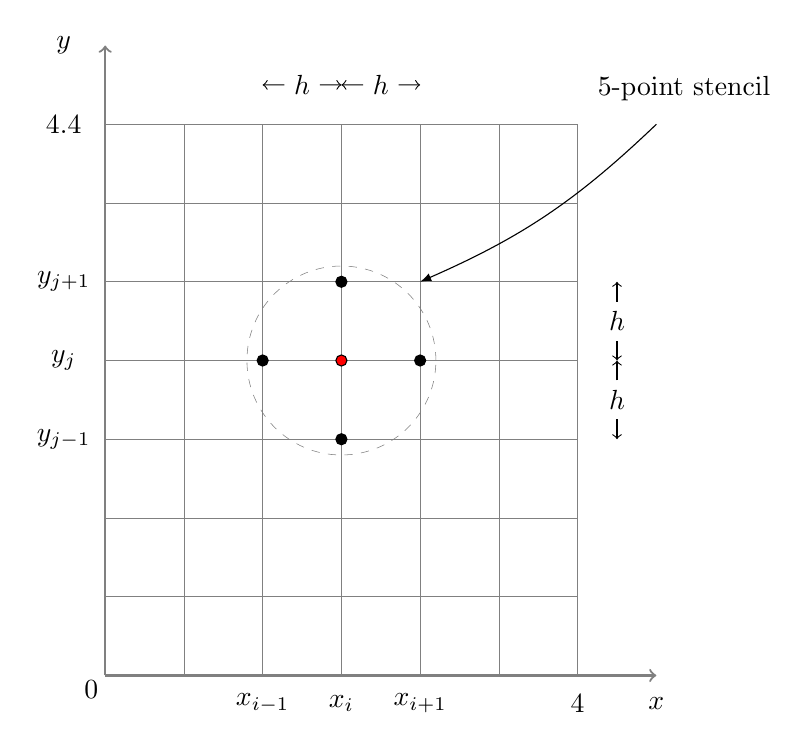
\begin{tikzpicture}
    \coordinate (Y) at (-15pt,8);
    \coordinate (X) at (7,-10pt);
    \draw[step = 1cm,gray, very thin] (0,0) grid (6,7);
    \draw[thick,color=gray,->] (0,0) -- (7,0);
    \draw[thick,color=gray,->] (0,0) -- (0,8);
    \draw (X) node {$x$};
    \draw (Y) node {$y$};
    \draw (X) node[shift={(-4,0)}] {$x_i$};
    \draw (Y) node[shift={(0,-4)}] {$y_j$};
    \draw (X) node[shift={(-5,0)}] {$x_{i-1}$};
    \draw (Y) node[shift={(0,-5)}] {$y_{j-1}$};
    \draw (X) node[shift={(-3,0)}] {$x_{i+1}$};
    \draw (Y) node[shift={(0,-3)}] {$y_{j+1}$};
    \draw (Y) node[shift={(0,-1)}] {$4.4$};
    \draw (X) node[shift={(-1,0)}] {$4$};
    \midlabelline{[shift={(-0.5,3cm + 10pt)}]X}{[shift={(-0.5,4cm +10pt)}]X}{$h$};
    \midlabelline{[shift={(-0.5,4cm +10pt)}]X}{[shift={(-0.5,5cm +10pt)}]X}{$h$};
    \coordinate (Xa) at ([shift={(2cm +15pt,-0.5)}]Y); 
    \coordinate (Xb) at ([shift={(3cm +15pt,-0.5)}]Y); 
    \coordinate (Xc) at ([shift={(4cm +15pt,-0.5)}]Y); 
    \midlabelline{Xa}{Xb}{$h$};
    \midlabelline{Xb}{Xc}{$h$};
    \draw (0,0) node[shift={(-5pt,-5pt)}] {$0$};
    \draw[fill=red] (3,4) circle (2pt) ;
    \draw[fill=black] (4,4) circle (2pt) ;
    \draw[fill=black] (2,4) circle (2pt) ;
    \draw[fill=black] (3,3) circle (2pt) ;
    \draw[fill=black] (3,5) circle (2pt) ;
    \draw[dashed,very thin,color=gray] (3,4) circle (1.2cm) ;
    \draw [latex-] (4cm,5cm) to [bend right=10] (7,7) node[anchor=south,shift={(10pt,5pt)}] {$5$-point stencil};
\end{tikzpicture}
\end{figure}
\noindent
Therefore we have,$U'_{i,j} = U'(x_i,y_j)$ and $\rho'_{i,j} = \rho'(x_i,y_j)$ $\forall \gs i \in \{0,1,\dots,N_x\} ; \gs j \in \{0,1,\dots,N_y\} $. \\[2mm] where $N_x = \frac{4}{h} $ and  $N_y = \frac{4.4}{h}$ \\[2mm]   
We replace the second-order derivatives in partial differential equation (2.16) with central difference operators,
\begin{align}
    &\delta^2_x U'_{i,j} + \delta^2_y U'_{i,j} = - \frac{\rho'_{i,j} s^2}{\epsilon_0 \nu} \\
    &\frac{1}{h^2}(U'_{i+1,j}+ U'_{i-1,j} -4 U'_{i,j} + U'_{i,j+1}+ U'_{i,j+1}) = - \frac{\rho'_{i,j} s^2}{\epsilon_0 \nu}
\end{align}

After rearranging we obtain the useful relation,
\begin{align} \label{eq:difference equation}
    U'_{i,j} = \frac{1}{4} \left[ U'_{i+1,j}+ U'_{i-1,j} + U'_{i,j+1}+ U'_{i,j+1} + h^2\frac{\rho'_{i,j} s^2}{\epsilon_0 \nu} \right] \\ \gs \forall \gs i \in \{1,2,\dots,N_x-1\} ; \gs j \in \{0,1,\dots,N_y\} 
\end{align}

The Dirichlet boundary conditions get translated to,
\begin{align*}
    U'_{i,j} = 5 \gs \forall \gs i \in \{0,N_x\} ; \gs j \in \{0,1,\dots,N_y\}
\end{align*}
and Neumann to,
\begin{align*}
    &U'_{i,j+1} = U'_{i,j-1} \gs \forall \gs j = N_y ; \gs i \in \{0,1,\dots,N_x\} \\
    &U'_{i,j-1} = U'_{i,j+1} \gs \forall \gs j = 0 ; \gs i \in \{0,1,\dots,N_x\} 
\end{align*}
\subsection{Iterative methods to solve linear algebraic equations}

In the last section we have discussed how to reduce a PDE to a linear combination of function values at various nodes by means of the method of finite differences. If we let the function value at any node as an unknown variable then the stencil when applied to all interior nodes gives rise to a system of linear algebraic equations, which may be very large. A two-dimensional problem like ours may lead to a system of several thousand unknowns, and three-dimensional problems involving several hundred thousand unknowns are common in real engineering situations. The solution of such a system is a major problem in itself as traditional methods like Gaussian-elimination result in large computation times, we are therefore forced to employ faster methods. As we have seen above, the system of equations produced by a discretisation has many special features and an efficient solution procedure must exploit these. The most obvious property of the system is that it is extremely sparse. Even when there are many thousand unknowns, each equation will involve one unknown and the unknowns at its immediate neighbourhood. In particular, if we write the equations in the conventional notation,
\begin{equation*}
    A \mvec{x} = \mvec{b} 
\end{equation*}
where A is an N × N matrix, b the given data vector and x the vector
of N unknown interior mesh values, there is an implied one-dimensional
ordering of these values which is somewhat unnatural and obscures the
important property that only immediate neighbours are involved. Each
row of the matrix A involves only a very small number of non-zero
elements, commonly five or seven; moreover in many problems a suitable
ordering of the unknowns will lead to a matrix in which these non-zero
elements occur in a regular pattern. In devising efficient methods for
the solution of the system these structural properties will be important,

\subsubsection{Jacobi Method}
\begin{algorithm}
	\caption{Jacobi Method}
	%{This iterative method takes an initial matrix of guess values and solves the the equation $$ Ax = b $$})
	\KwData{INPUT -: An $ k \times m $ matrix of initial values, value of step size $h$ and  also a matrix containing the initial charge configuration} 
	\KwResult{OUTPUT -: An $ k \times m $ matrix containing the values of potential on all $x$ and $y$ values} 
	\For{f = 0, 1, 2, 3, 4....N}{ 
		make new array of size $ k \times m $ \tcc*{initialising a new array for solution}
		\For(\tcc*{taking a x value}){i =0, 1, 2, 3 ... k}{
			\For(\tcc*{taking all y value for a x value}){ j =1, 2, 3 ... (m-1)}{
				\tcc{now defining the required quantites for stencil}
				$left = {a}_{i,j-1}$ \; 
				$right = {a}_{i,j+1}$ \;
				\If{$ i = k-1 $ }{
					$up = {a}_{i-1,j}$\;
					\Else{
						up = ${a}_{i+1,j}$\;
						
					}							
				}
				\If{ $ i = 0 $}{
					down = ${a}_{i+1,j}$\;
					\Else{
						down = ${a}_{i-1,j}$ \;
					}
				}
				{new ${a}_{i,j}$ = (up + down + left + right + $h^2 * {p}_{i,j} $ )/4 + new ${a}_{i,j}$} \tcc*{new value the grid point}
			}
			{max relative error = max(new  x - x)/ $x$}\;
			\If(\tcc*{checking for tolerance}){max relative error < tolerance}{
				{break}\;
				\Else(\tcc*{if tolerance not reached then the iteration continues}){
					new x =  x	
				}
			}
		}
	}	
\end{algorithm}
\subsubsection{Gauss-Seidel Method}
\subsubsection{Relaxation methods and Successive Over-Relaxation(SOR)}



\newpage

\section{Numerical Analysis}
Although one certainly would have some intuition about how the potential distribution should look like if the distribution had lesser number of charge distributions, the intuition tends to be not so reliable in complex systems. Therefore it becomes natural to approach computaional methods for help. The computaional results themselves have to be judged, one way to do so is a brief check that the result vaguely approximates our intuition, another method is by employing different computaional methods to make sure that the method is not biased to a particular solution. For example, if SOR produces a wildly different solution than Jacobi or the former takes more number of iterations than later then certainly either one of the solvers is wrongly implemented. Before we move on to analysing the various results we obtained using the different solving methods, we will first establish the intuitive expectations that we first put forward while framing the problem and before obtaining the final results. Later we will have a short discussion about the role discritization plays in our solution.

\subsection{Expectations}

To remind ourselves, our problem consists of an interleaved capacitor which is charged to a potential of $\pm5 V$ and then disconnnected. In our problem the first plate $A_{1}$ and the last plate $A_5$ of the capacitor were maintained at $+5V$. We are solving our problem assuming perfect symmetry along the third direction that is along the surface of the plates.(the z-direction).

\begin{figure}[ht]
    \centering
    \def\svgwidth{0.6\textwidth}
    \import{../diagrams}{analysis.pdf_tex}
    \caption{This diagram represents the region $\omega$ being studied, $\alpha_1,\alpha_2,\alpha_3,\alpha_4$ are the only unique regions in $\omega$ that were analysed.}
    \label{}
\end{figure}
\begin{itemize}
    \item \textbf{Symmetry: } Now since in our arrangement is symmetrical, the resulting solution obtained should also be symmetrical about the line $x = 2$. 
    \item High Potential near the positively charged plates (i.e. the plates denoted by A  in the figure1) of capacitor and low potential near the negatively charged plates but we are considerig them in two dimension so they will behave as the "line charge distributions. Since we are ensuring the value at the boundary reamins constant at $ +5 volts $ so the distribution should contain a positive spike in value of potential at the location of $A_i$  having positive potential at the beginning and negative spike at places of negative potential
    \item  In region $ \alpha_2 $ potential is fixed at $ + 5 volts $ at $ x = 0 $ and stretches to $ x = 0.5 $ where $ B_1 $ was initially charged with $ - 5 volts $. We expect to see a decline in potential in region $ \alpha_2 $ due to initial conditions across x direction.
    \item The  $ B_1 $ plate extends for $ y \in (0.4, 4.4)  $ so we expect to see concentration of negative charges hence negative potential  for  higher values  of y where initially there was presence of negatively charged potential plate $ B_1 $ and a comparitively higher potential for $ \alpha_1 $ or lower values of y because it is surrounded by two positively charged plates.
    \item for region $ \alpha_3   $  we expect to see a rise  in potential from $ x = 0.5 $ to $ x = 1 $  because it is surrounded by negatively charged potential plate at $ x = 0.5 $ and postively charged plate at  $ x = 1 $.
    \item The plate $ A_2 $ ends at the boundary of $ \alpha_4 $ and it is surrounded by two negatively charged plates on both sides so we expect to see a concentration of negatively charged potential in region $ \alpha_4 $.
    \item For region $ x \in (1 , 1.5) $ the trend should be similar to region $ \alpha_2 $ and for region $ x \in (1.5, 2) $ we expect  trend to be similar to $ \alpha_4 $ . 
    \item Now due to symmetry we expect to see the potential distribution after $ x = 2 $ same as before it with the line $ x = 2 $ as mirror
\end{itemize}

\subsection{Results}
Now that we have converted the problem into a system of linear equations by applying the relation \ref{eq:difference equation} to each node on the mesh and analysed the conversion, we move on to analyse the computational results obtained using three different iterative methods namely Jacobi, Gauss-Seidel and S.O.R to solve the system of linear equations.


\begin{figure}[ht]
    \centering
    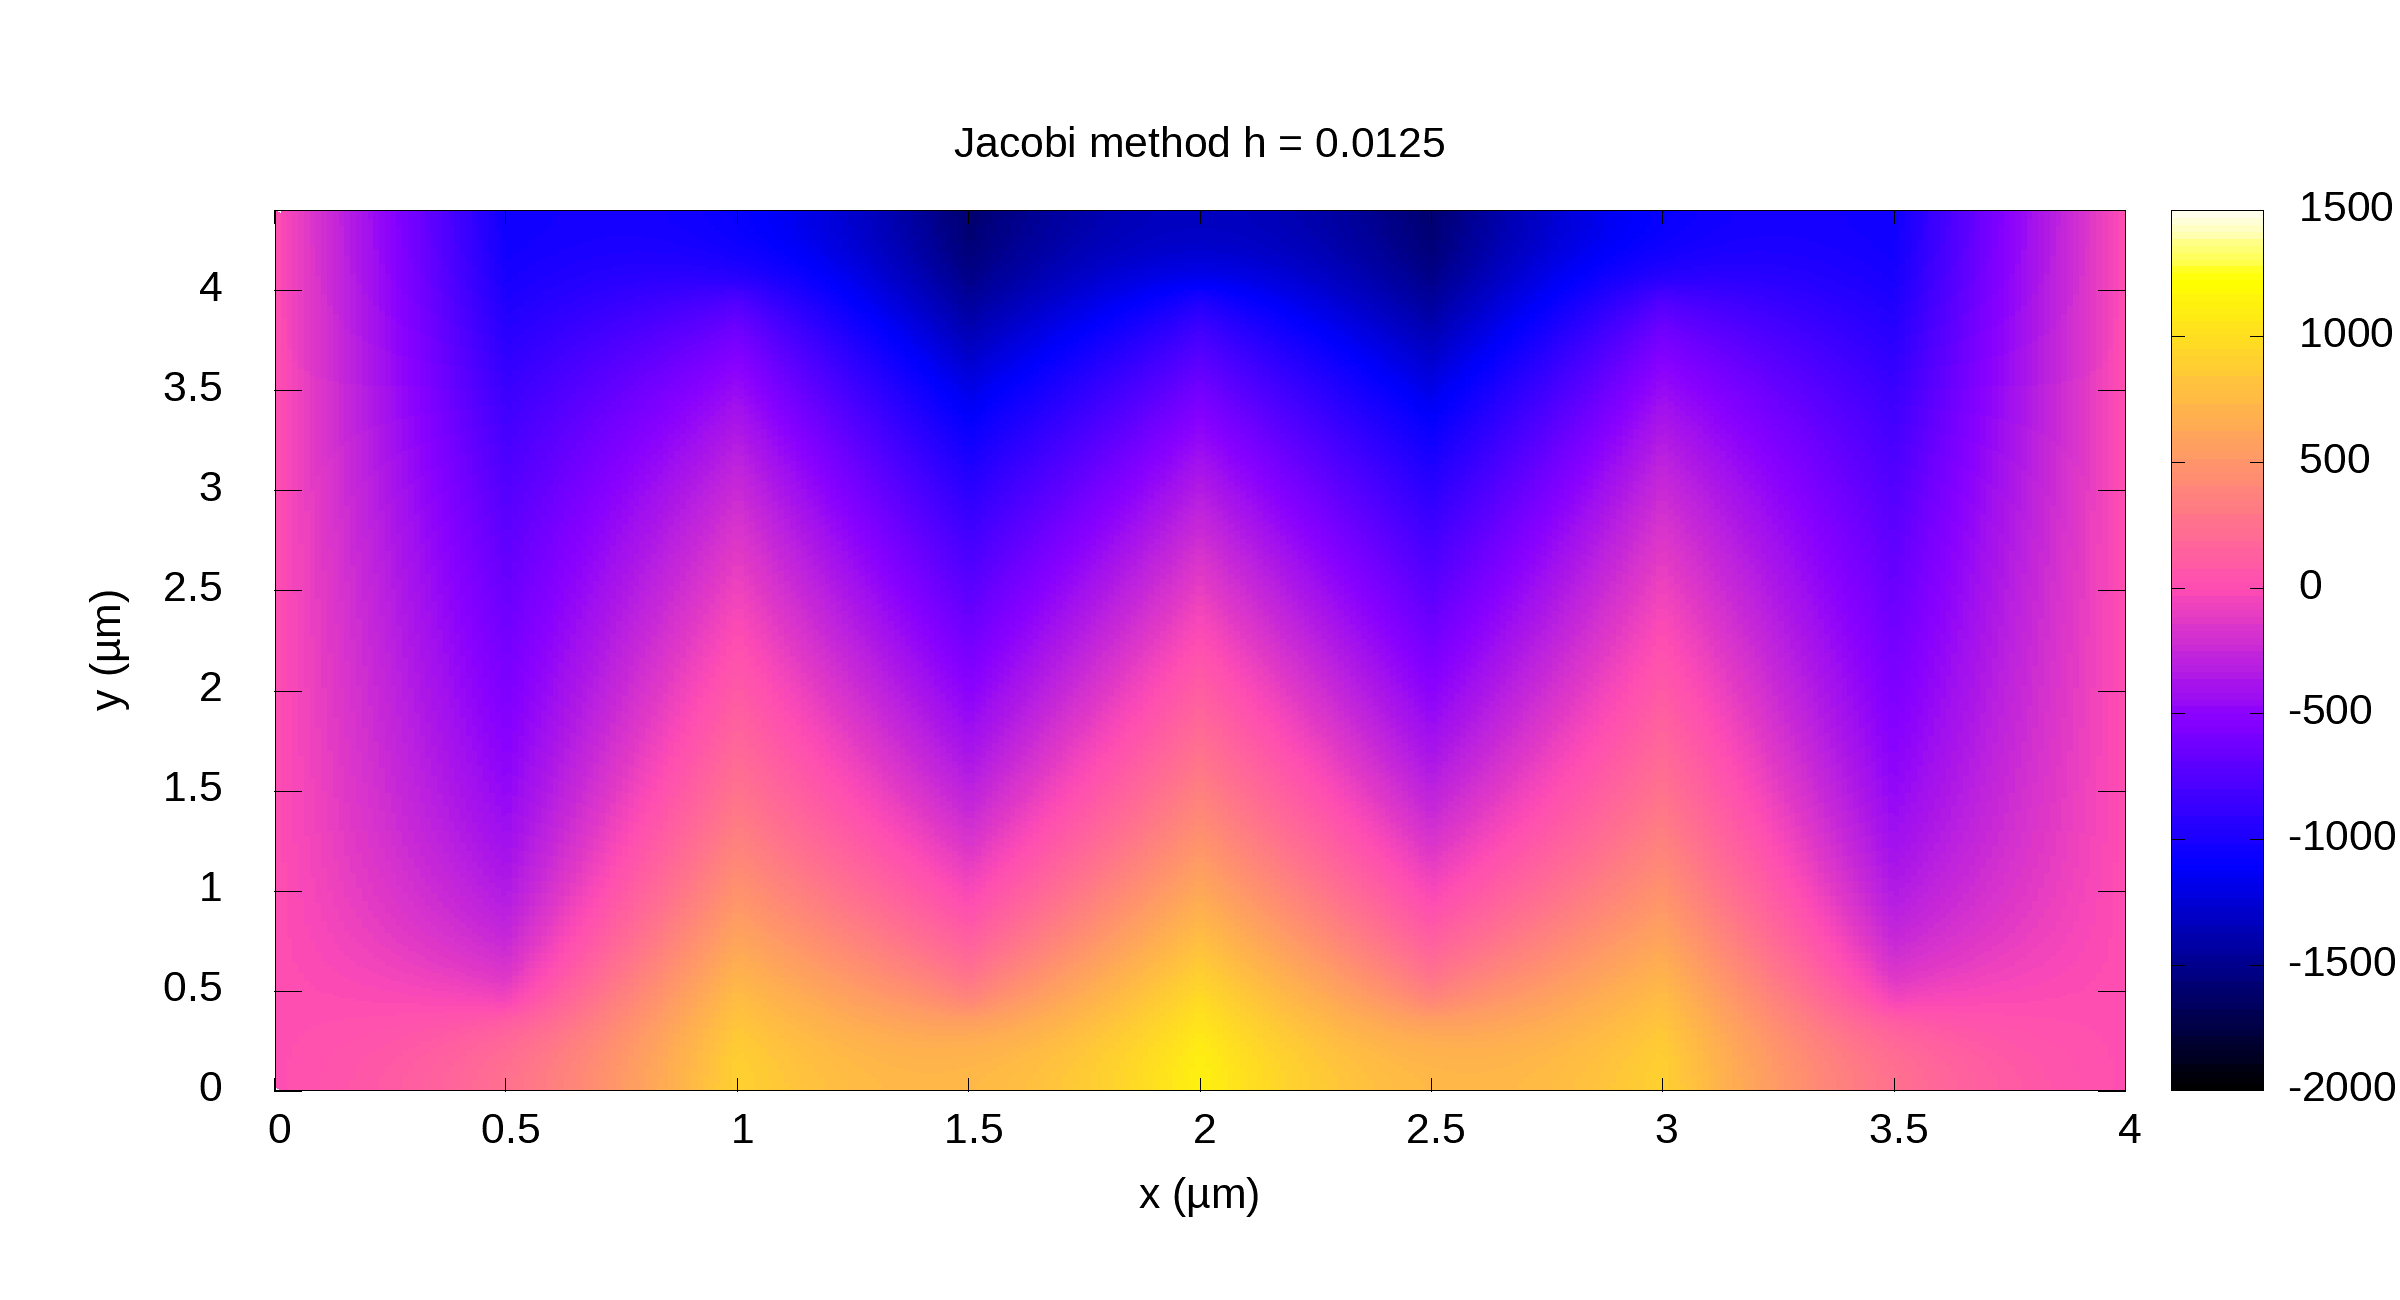
\includegraphics[height= 70mm]{content/graphs/Jacobi_0125_map.png}
    \caption{Jacobi}
    \label{fig1}
\end{figure}%

\begin{figure}[ht]
    \centering
    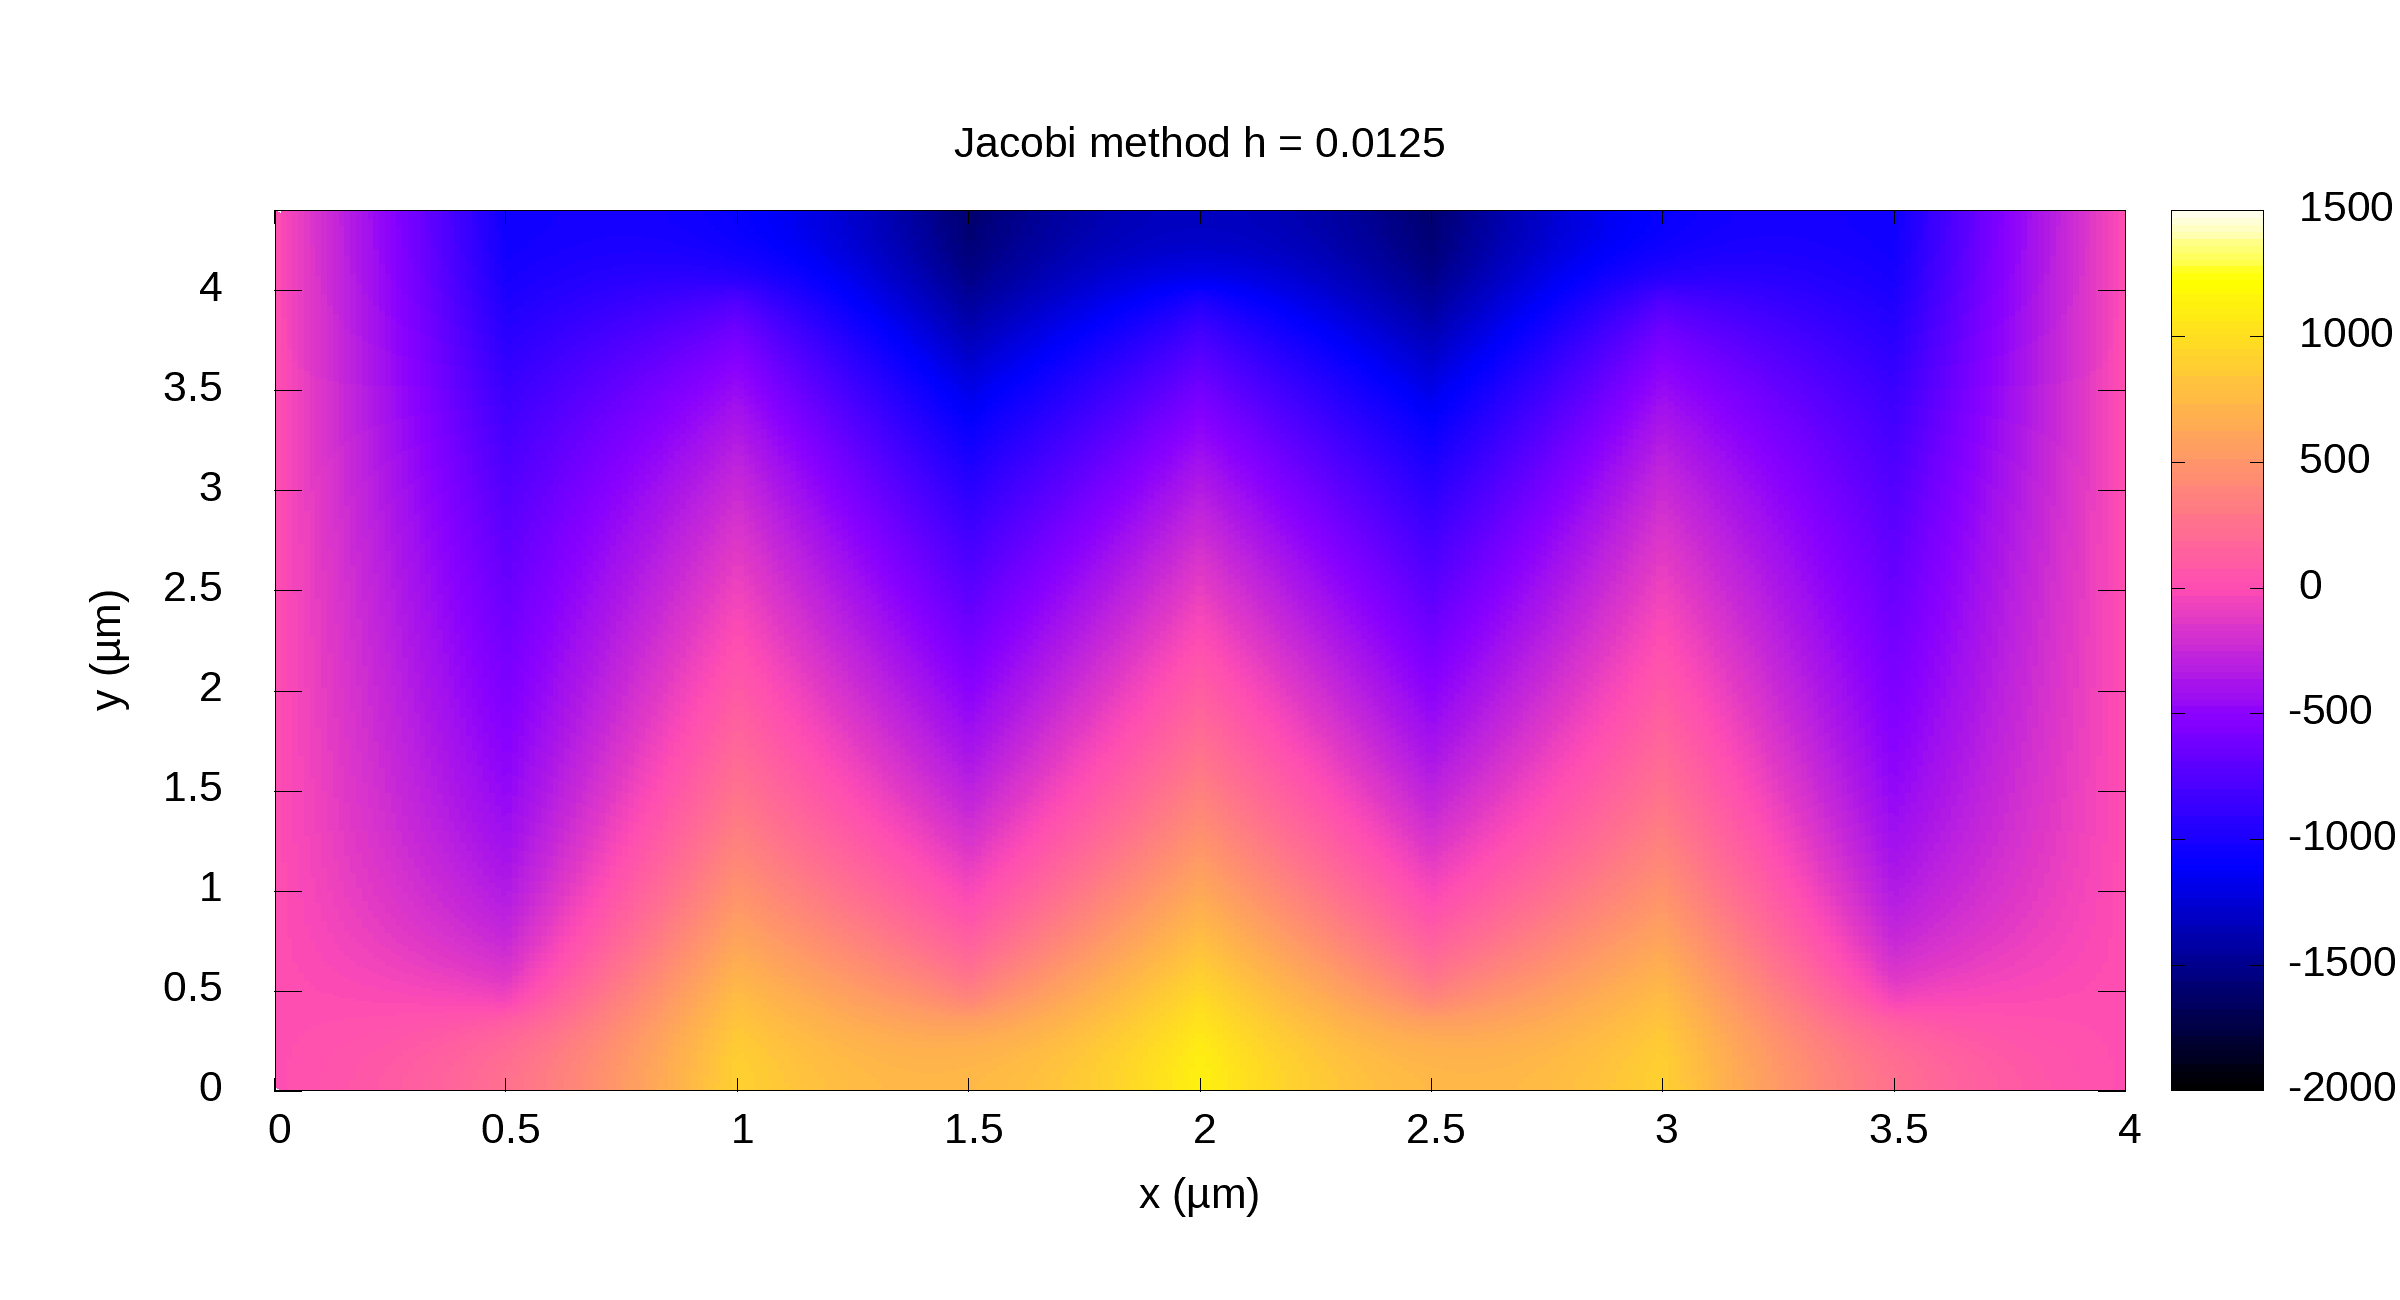
\includegraphics[height= 70mm]{content/graphs/Jacobi_0125_map.png}
    \caption{Jacobi}
    \label{fig2:}
\end{figure}%
\begin{figure}[ht]
    \centering
    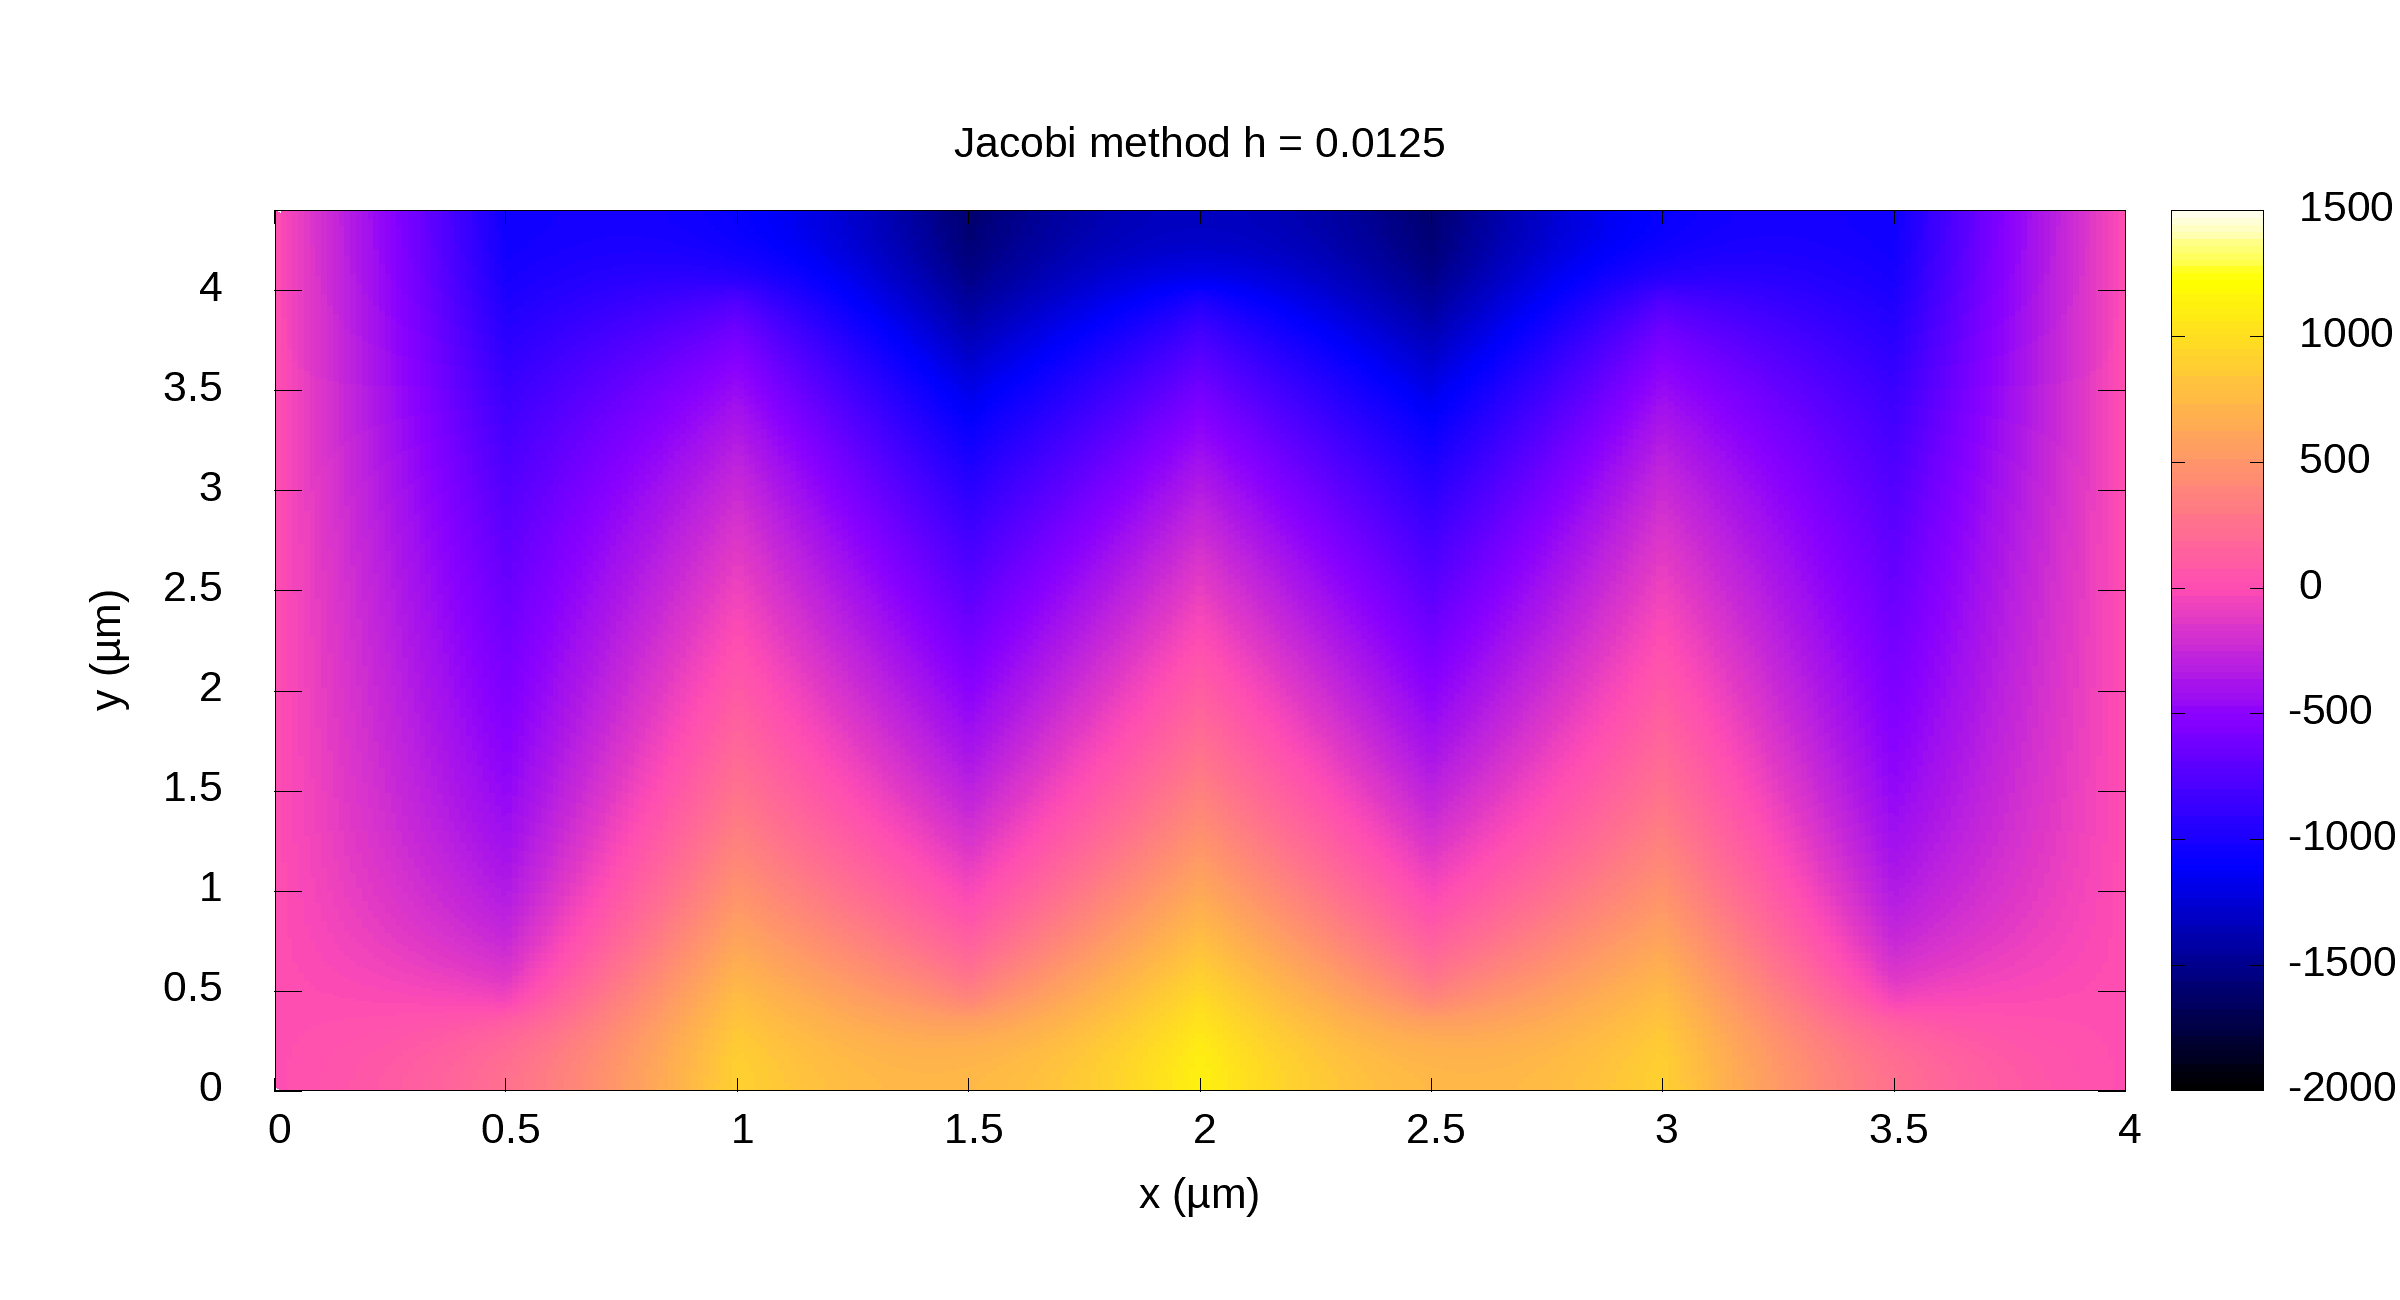
\includegraphics[height= 70mm]{content/graphs/Jacobi_0125_map.png}
    \caption{Jacobi}
    \label{fig3:}
\end{figure}%

\paragraph{Comparison of Method}{%
Since all the iterative methods we used have given us almost identical results so we will only compare them on the basis of number of iteration required so as to determine which method is more compuationally cheap and viable}
    
\begin{table}[ht]
    \centering
    \begin{tabular}{|c|c|c|c|}
    \hline
    \multirow{2}{*}{\gs\gs meshsize $h$ \gs\gs} & \multicolumn{3}{c|}{No. of iterations}  \\ \cline{2-4}
                                    & \gs \gs Jacobi \gs \gs & \gs \gs Gauss-Seidel \gs\gs & \gs S.O.R (1.9) \gs \\ \hline
    0.01                                &11878& 6315& 251\\ \hline
    0.05                                &52047& 26983 &1552\\ \hline
    0.025                               &182367&94927&5821\\ \hline
    0.0125                              &674230&335520 &22163 \\ \hline
\end{tabular}
\caption{\centering Table comparing the number of iterations required for each method for a relative tolerance of $10^{-8}$}
\label{iterations}
\end{table}


\begin{table}[ht]
    \centering
    \begin{tabular}{|c|c|c|c|}
    \hline
    \multirow{2}{*}{\gs\gs meshsize $h$ \gs\gs} & \multicolumn{3}{c|}{Approximate computation time ($\pm 0.01s$)}  \\ \cline{2-4}
                                    & \gs \gs Jacobi \gs \gs & \gs \gs Gauss-Seidel \gs\gs & \gs S.O.R (1.9) \gs \gs   \\ \hline
    0.01                                &0.41&0.27&0.02\\ \hline
    0.05                                &6.13& 3.96&0.28\\ \hline
    0.025                               &90.73&55.46&3.47 \\ \hline
    0.0125                              &1380.54&818.68&54.35\\ \hline
\end{tabular}
\caption{\centering Table comparing the computation time required for each method for a relative tolerance of $10^{-8}$}
\label{computation_time}
\end{table}

So comparing all the method for computation under identical condition on the basis of number of iteration required for acheiving the required tolerance we can say $ \boldsymbol{SOR Method} $ is best method among all three iterative schemes used.

\subsubsection{Successive Over Relaxation (SOR)}
In this section we analyse the results obtained for different values of relaxation factor. \\[2mm]
\noindent
\textbf{ Optimum value of Relaxation Factor } \\
In Successive Over Relaxation we have to choose the value of a relaxation factor which is responsible for the rate of convergence of solution. It's value can be chosen anywhere between 1 to 2 i.e. relaxation factor or $\omega  \in [1,2]$. We observed the variation of No. of iterations required to reach a given tolerance with change in $ \omega $. The following graph represents the graph between number of itereations and value of $\omega$. \\
\begin{figure}[ht]
    \centering
    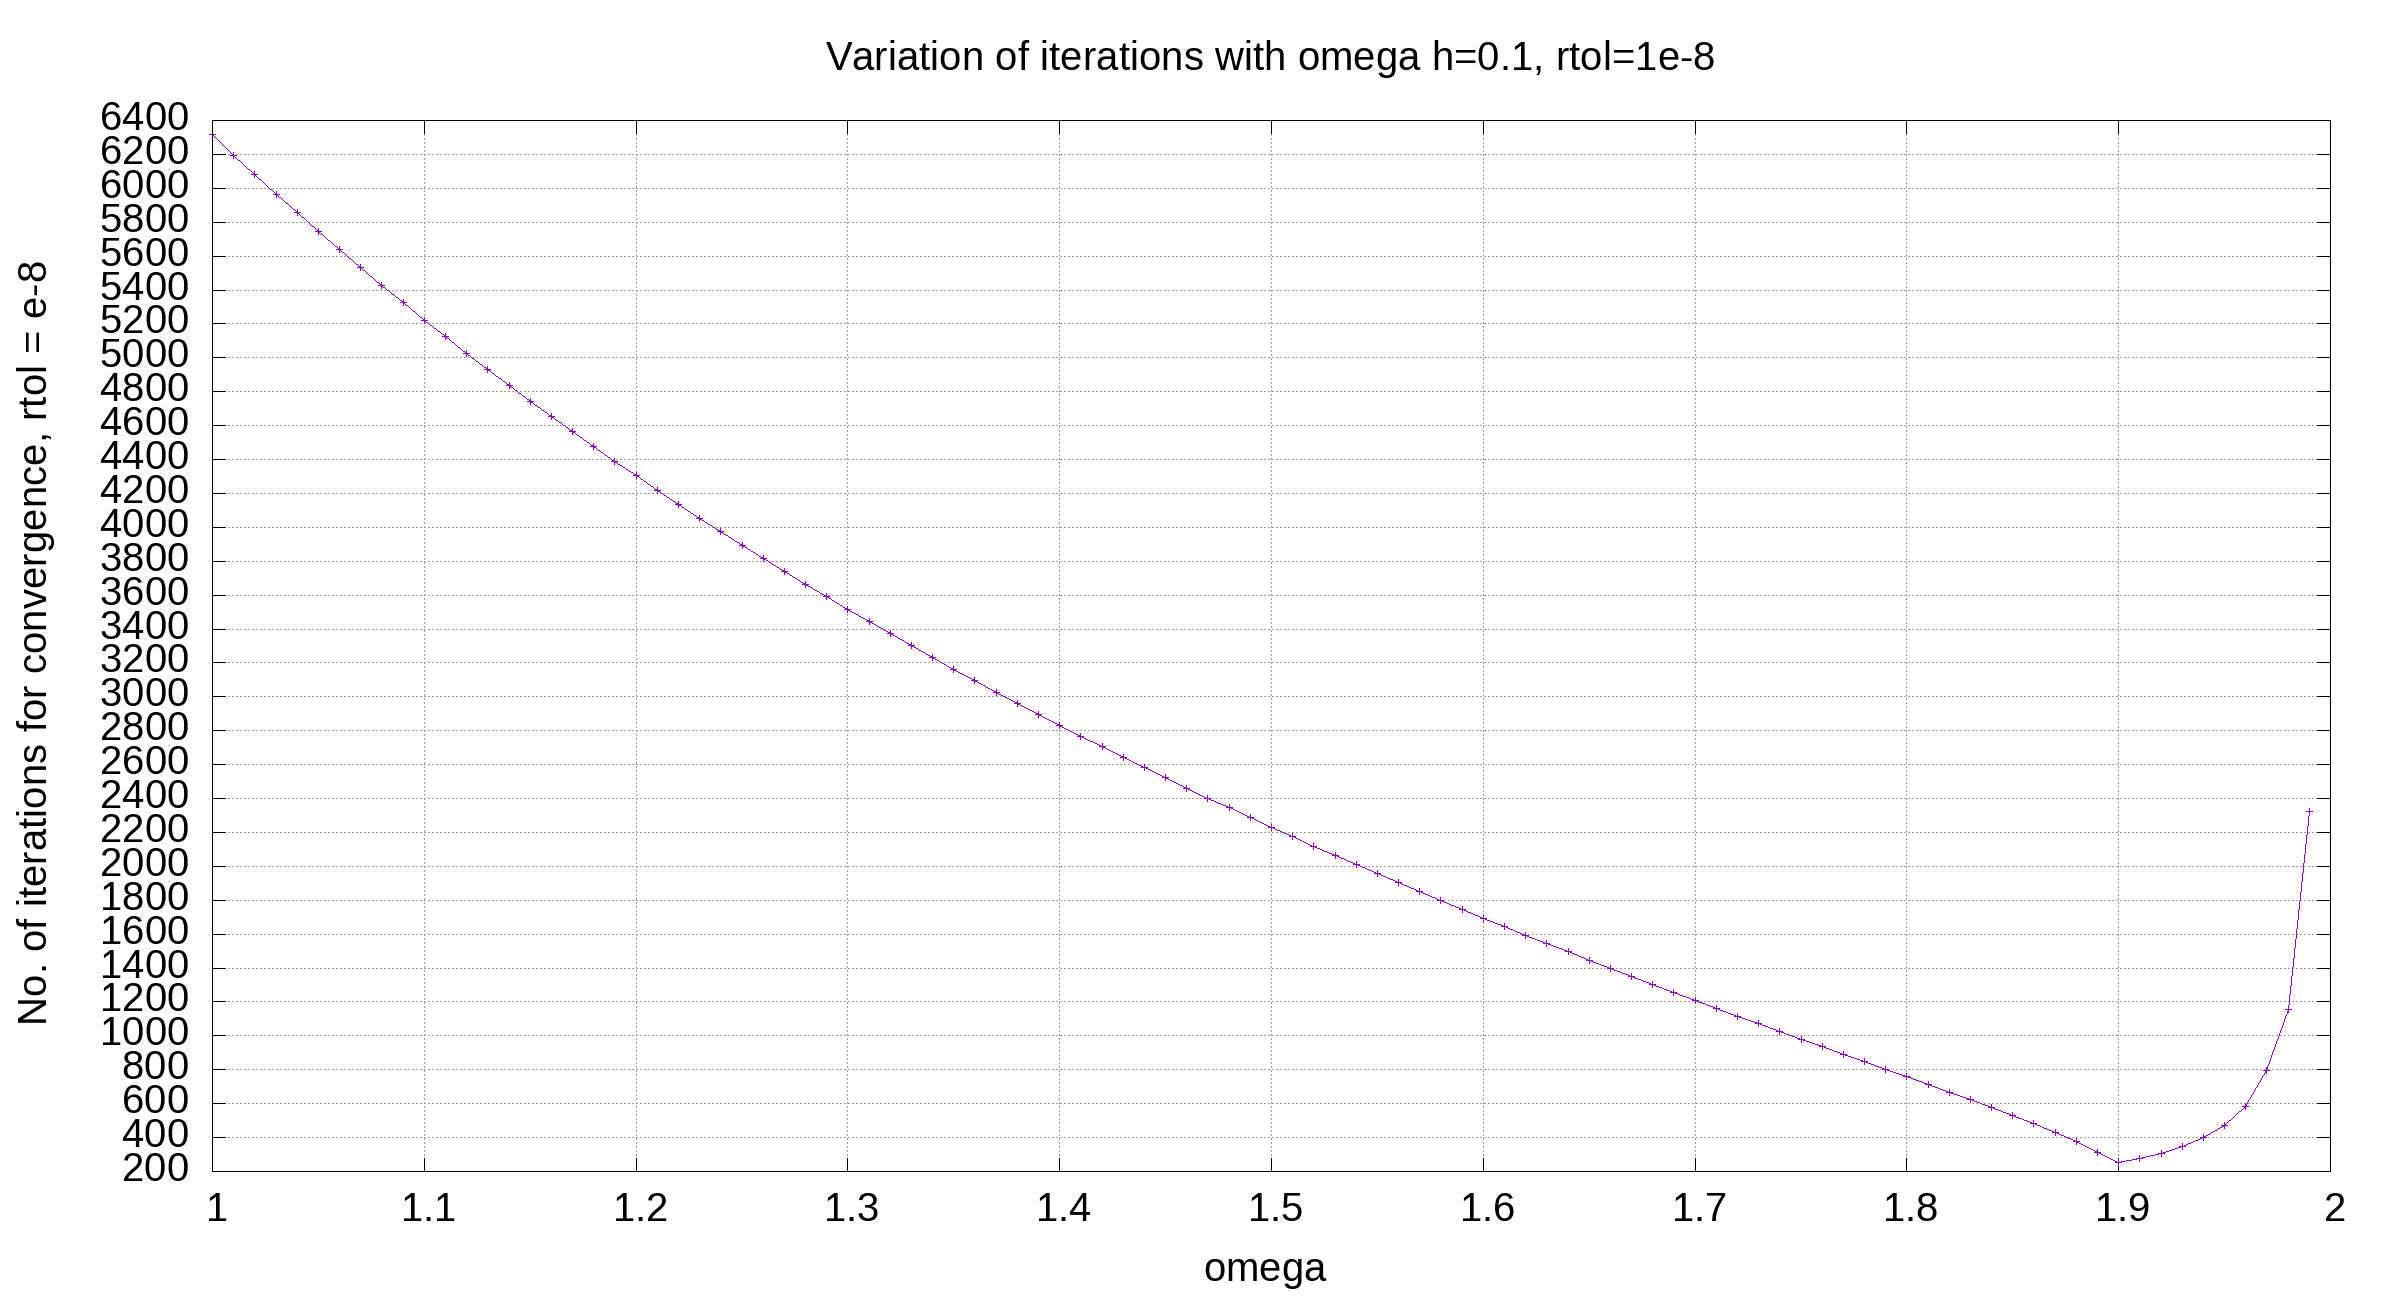
\includegraphics[width=\textwidth]{content/graphs/omega.png}
    \caption{variation of number of iterations for convergence with relative tolerance=$10^{-8}$ and meshsize $h = 0.1$  }
    \label{omega variation}
\end{figure}
From the graph we can see that the most optimum value of $ \omega $ is $1.89$ according to number of iterations required to reach the solution.


\newpage
\section{Conclusion}
\subsection{Result}
We tried to solve the problem of interleaved capacitor using the finite difference method for solving poisson equation. We have solved the problem using three different iterative schemes. After completing this project we can say that the method of SOR is best for solving the system of linear equation after using the finite differences method. Using SOR method we were able to solve mesh of size $ (480 times 480) $ in just $ xxxxxx $ number of iteration in just $  yyyy $ seconds. Also we gained good insight and intuition after solving the problem of interleaved capacitor.
\subsection{Experience}
We learnt a lot of new things during this project. We have gained the knowledge on how to solve a physical problem computationally and the various process involved in it such as non-dimensionalisation, the concept of convergence etc. Our python, latex and gnu skills have also increase significantly and our fascination with power of poisson equation and computation method have only gone uphill as compared to start of project of how one can solve such complex physical problem just by using some standard method and understand the "physical aspect " of such problems easily. We also spend a good portion of time studying about theoretical aspects of different computational methods and trying to understand the concepts about which we didn't pay a lot of attention to earlier such as the truncation error , round off error etc. This project has been an incredible journey for us as it has not only increased our theoretical , physical and compuational knowledge but it has also taught us about the importance of perseverance and patience as there were many topic or subtopics that we didn't understand easily just by studying about it from one or two place or things that were not easily available in comprehendable nature for us due to advance nature of partial differential equation and sometimes we have to spend a lot of time just searching about it. But in the end we are very grateful that we had chosen such a topic that has taught us so much. 

\newpage
\section{Appendix}
    \subsection{Non-Dimensionalization}
    
    \subsection{Programs}
    \subsection{Contributions}


\end{document}